% !TEX root = ../main.tex
\begin{figure}[h!]
\centering
\vspace{-0.1in}
\iflatexml
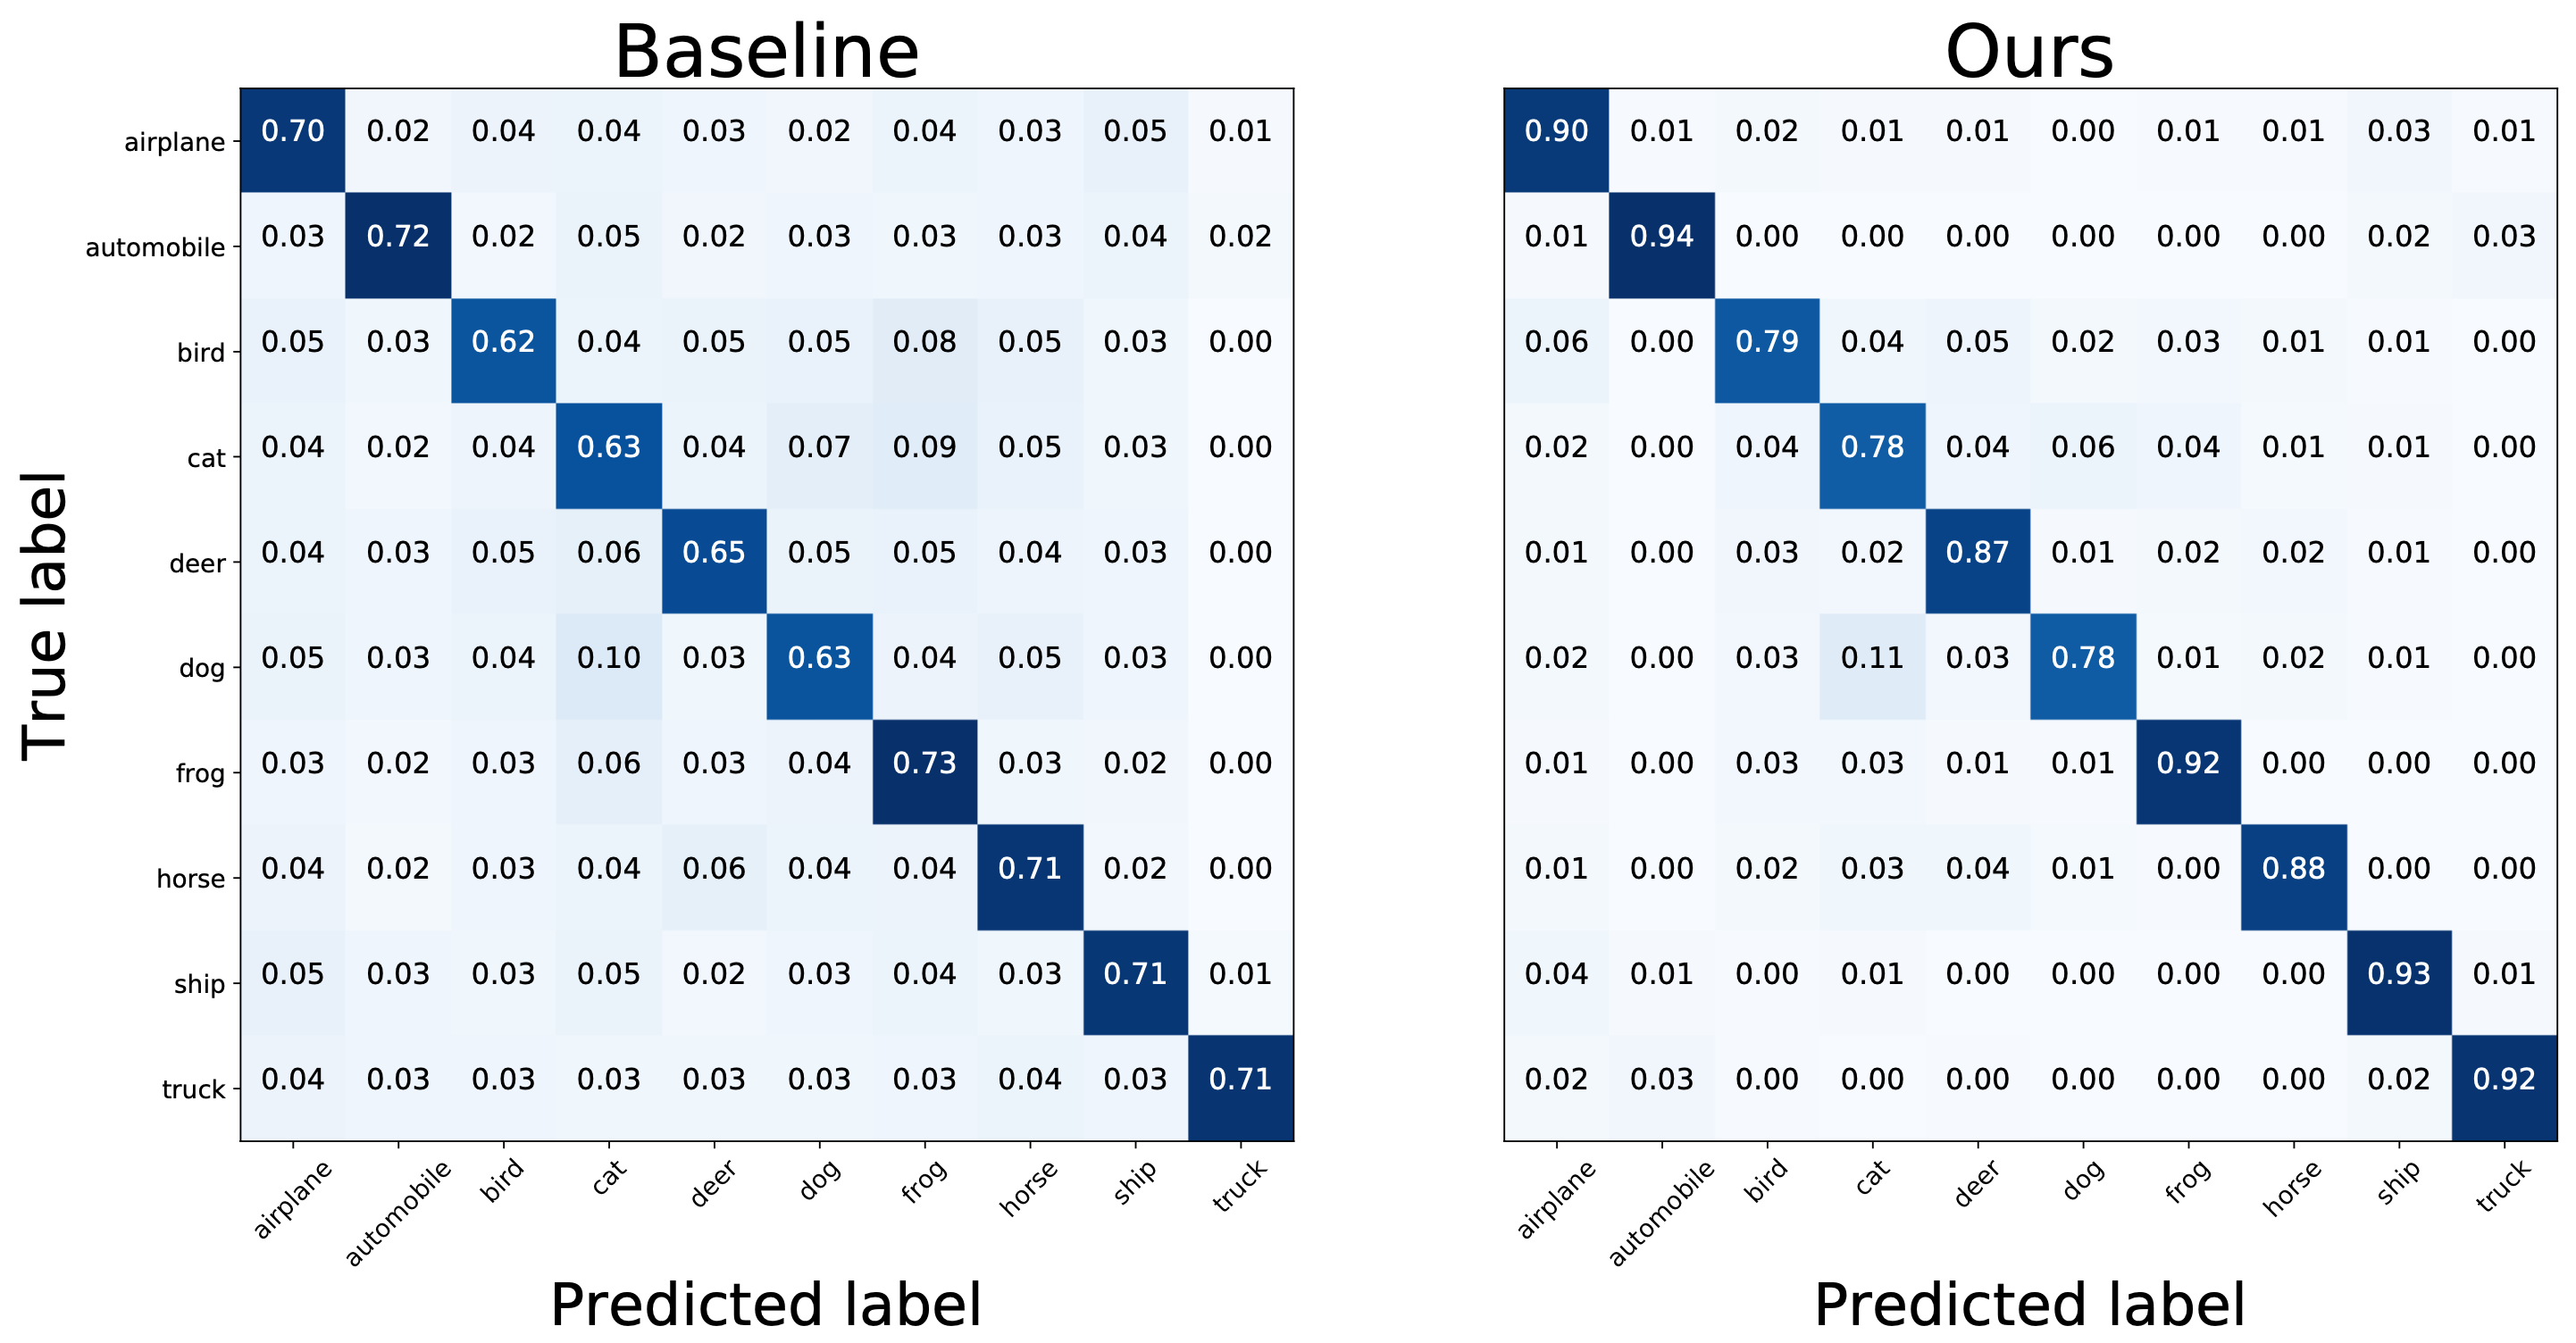
\includegraphics[width=3\columnwidth]{figures/cifar-noise-cm.png}
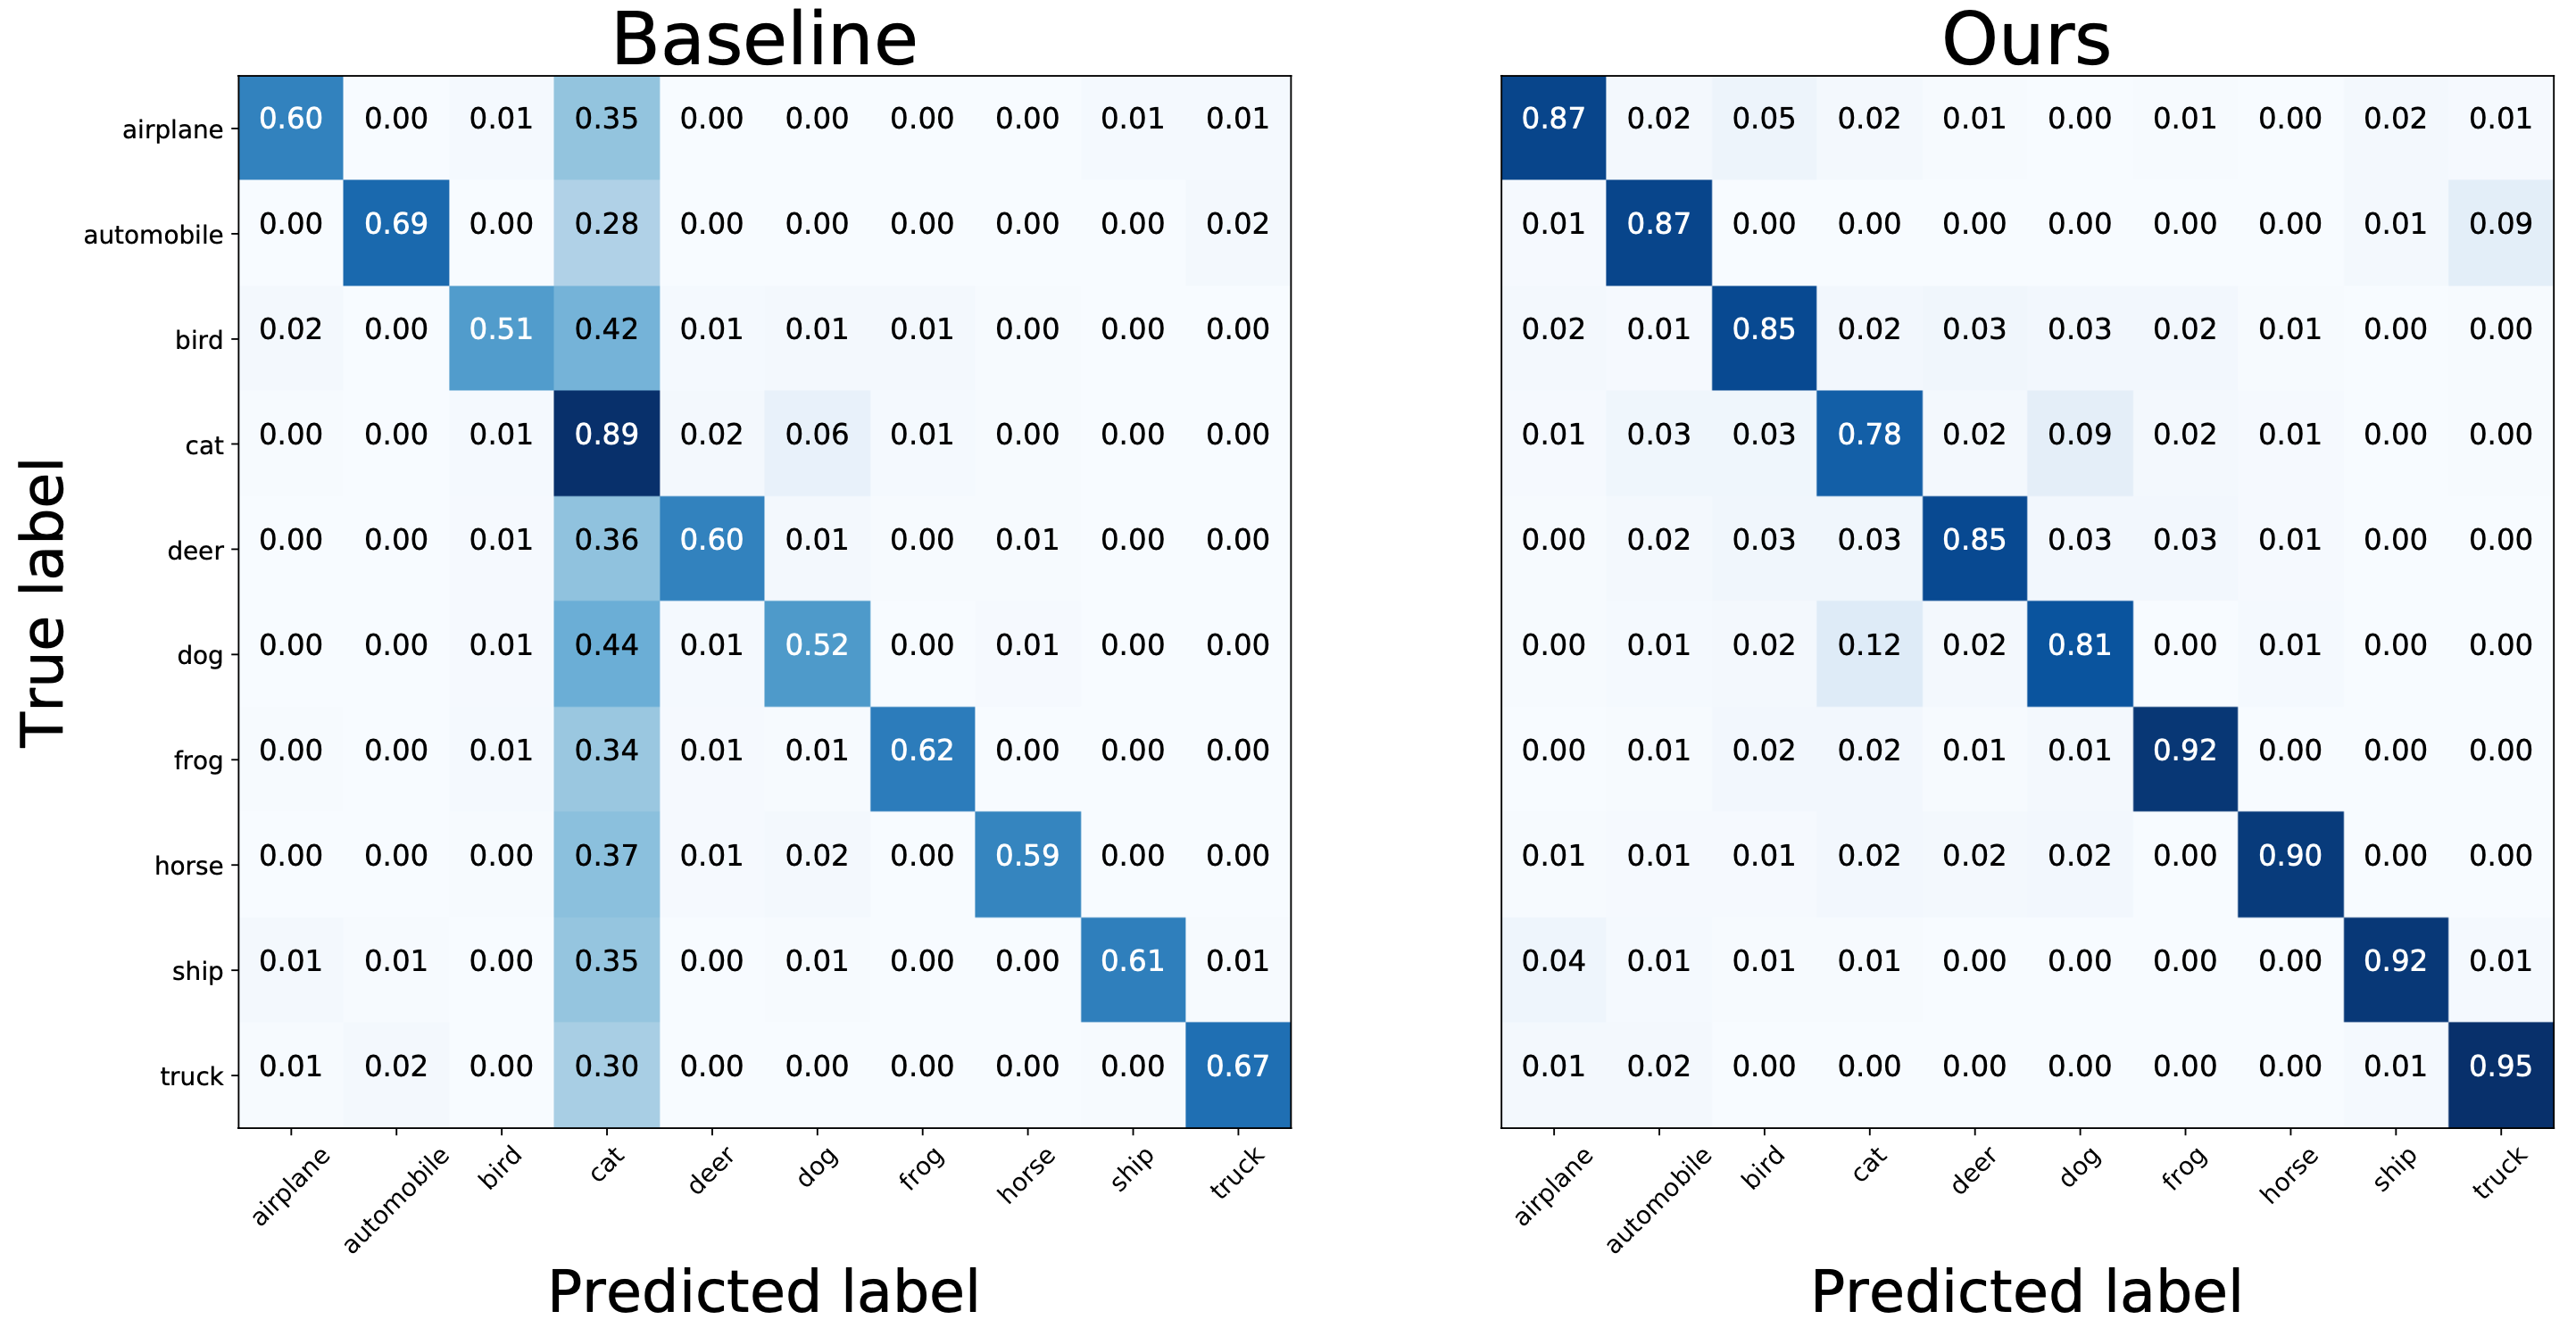
\includegraphics[width=3\columnwidth]{figures/cifar-imbalance-cm.png}
\else
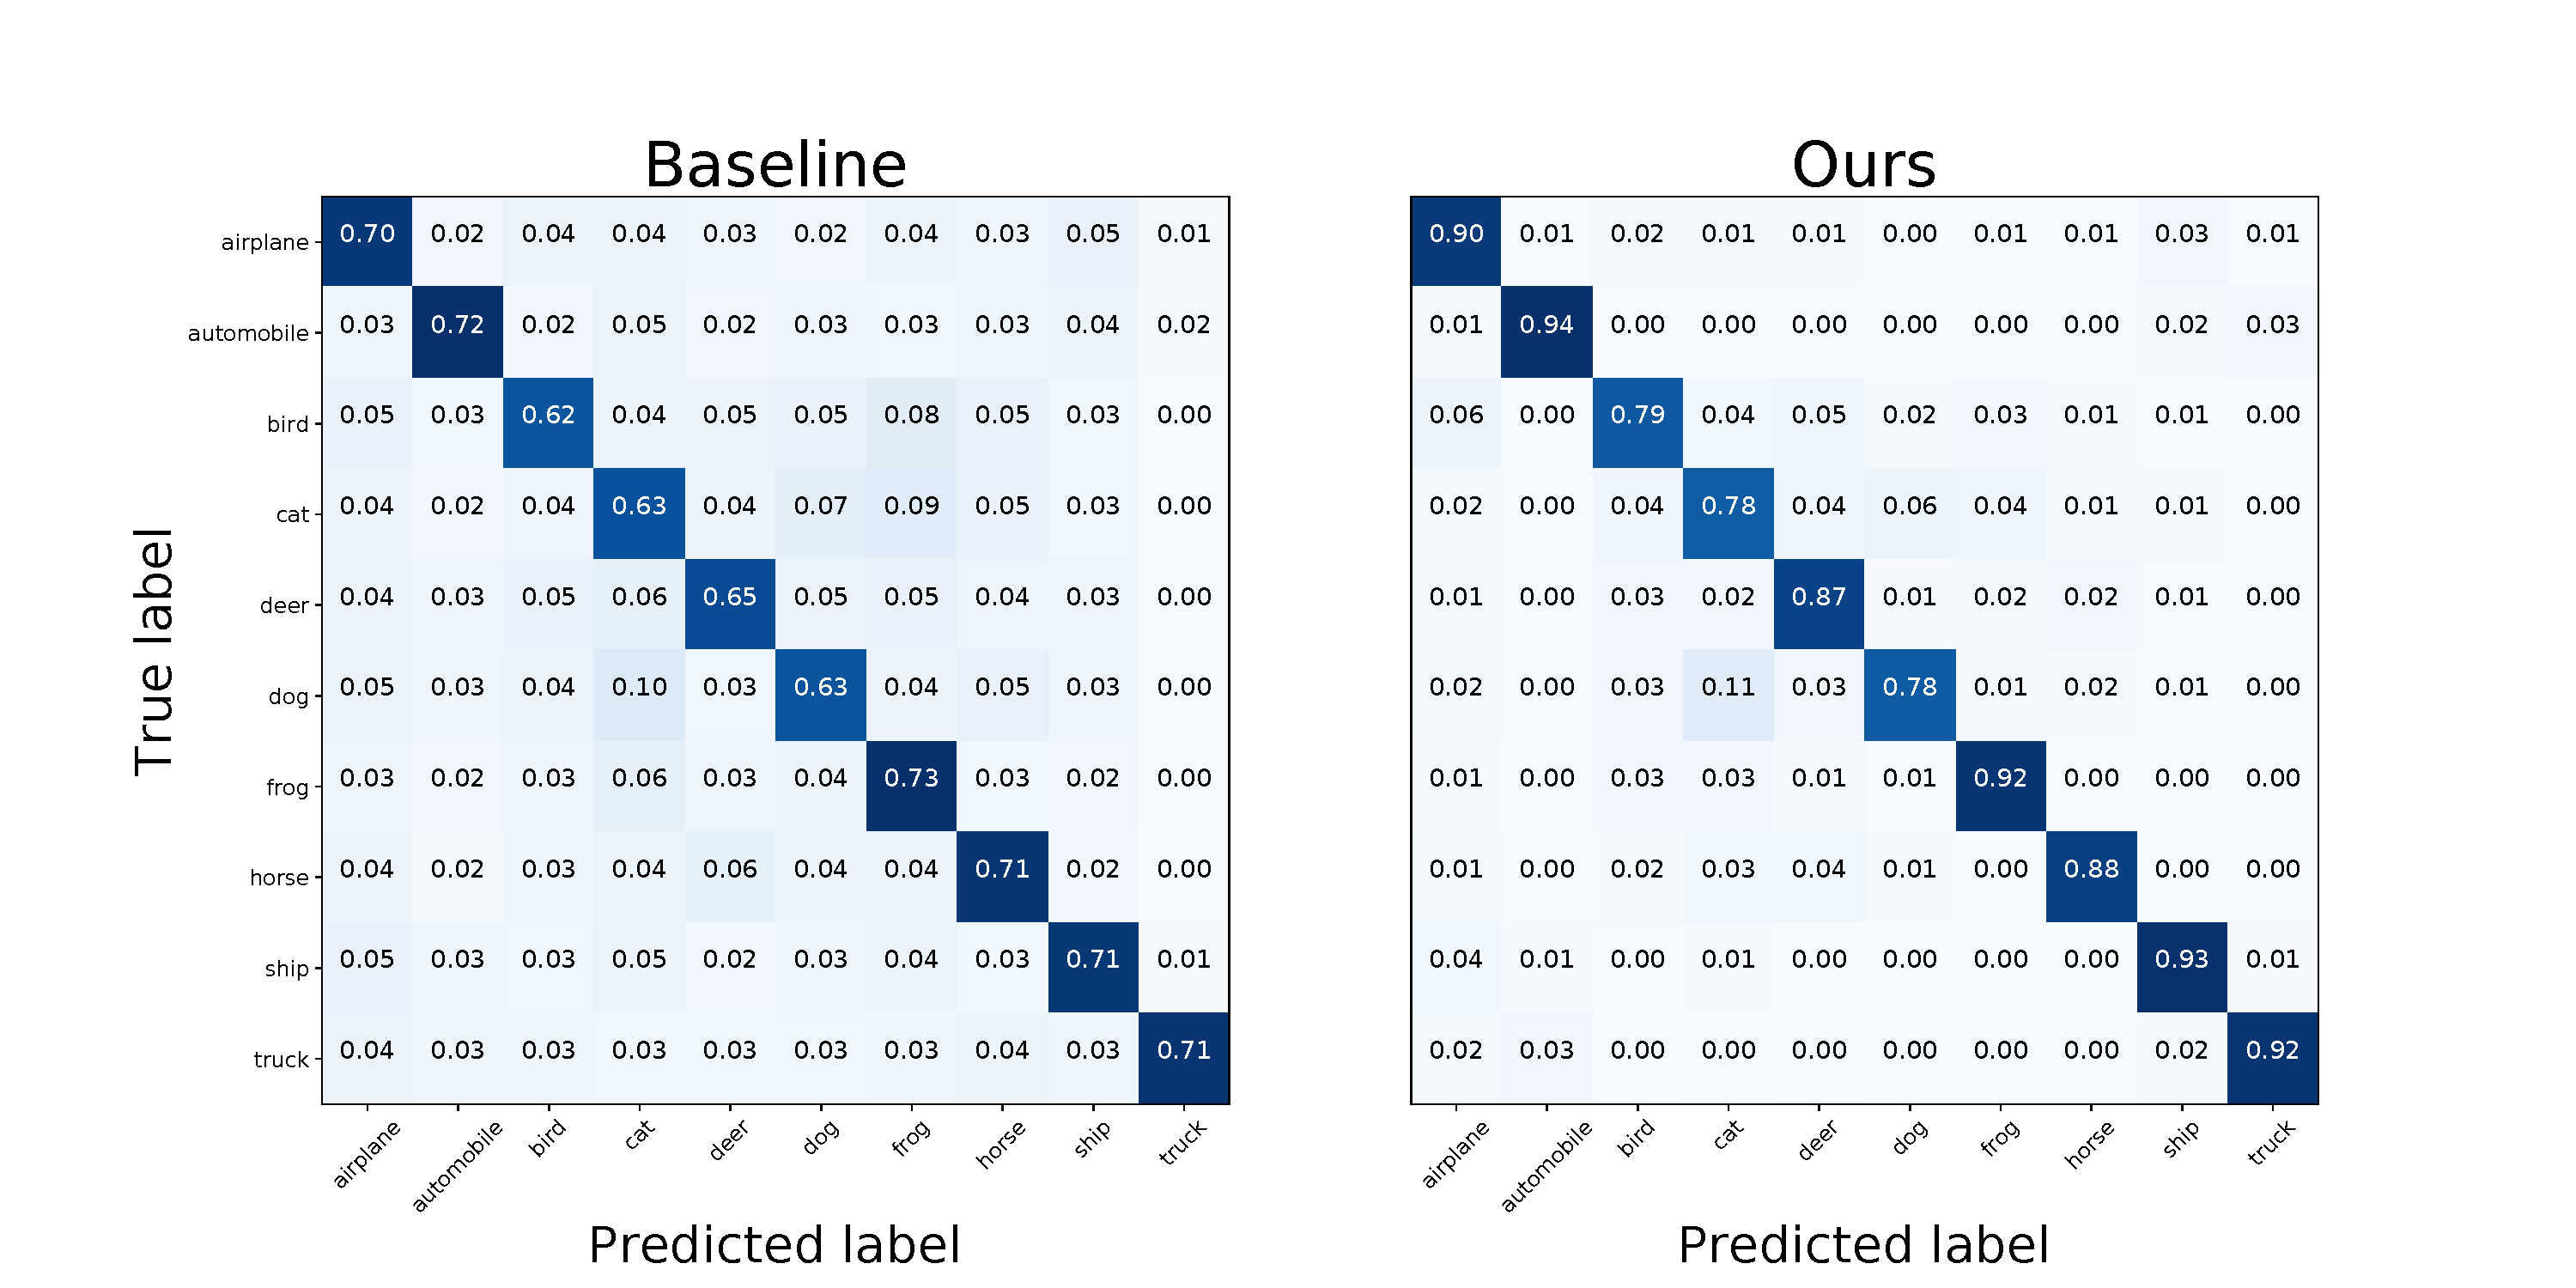
\includegraphics[width=\columnwidth,trim={2.5cm 0 4cm 0},clip]{figures/cifar-noise-cm.pdf}
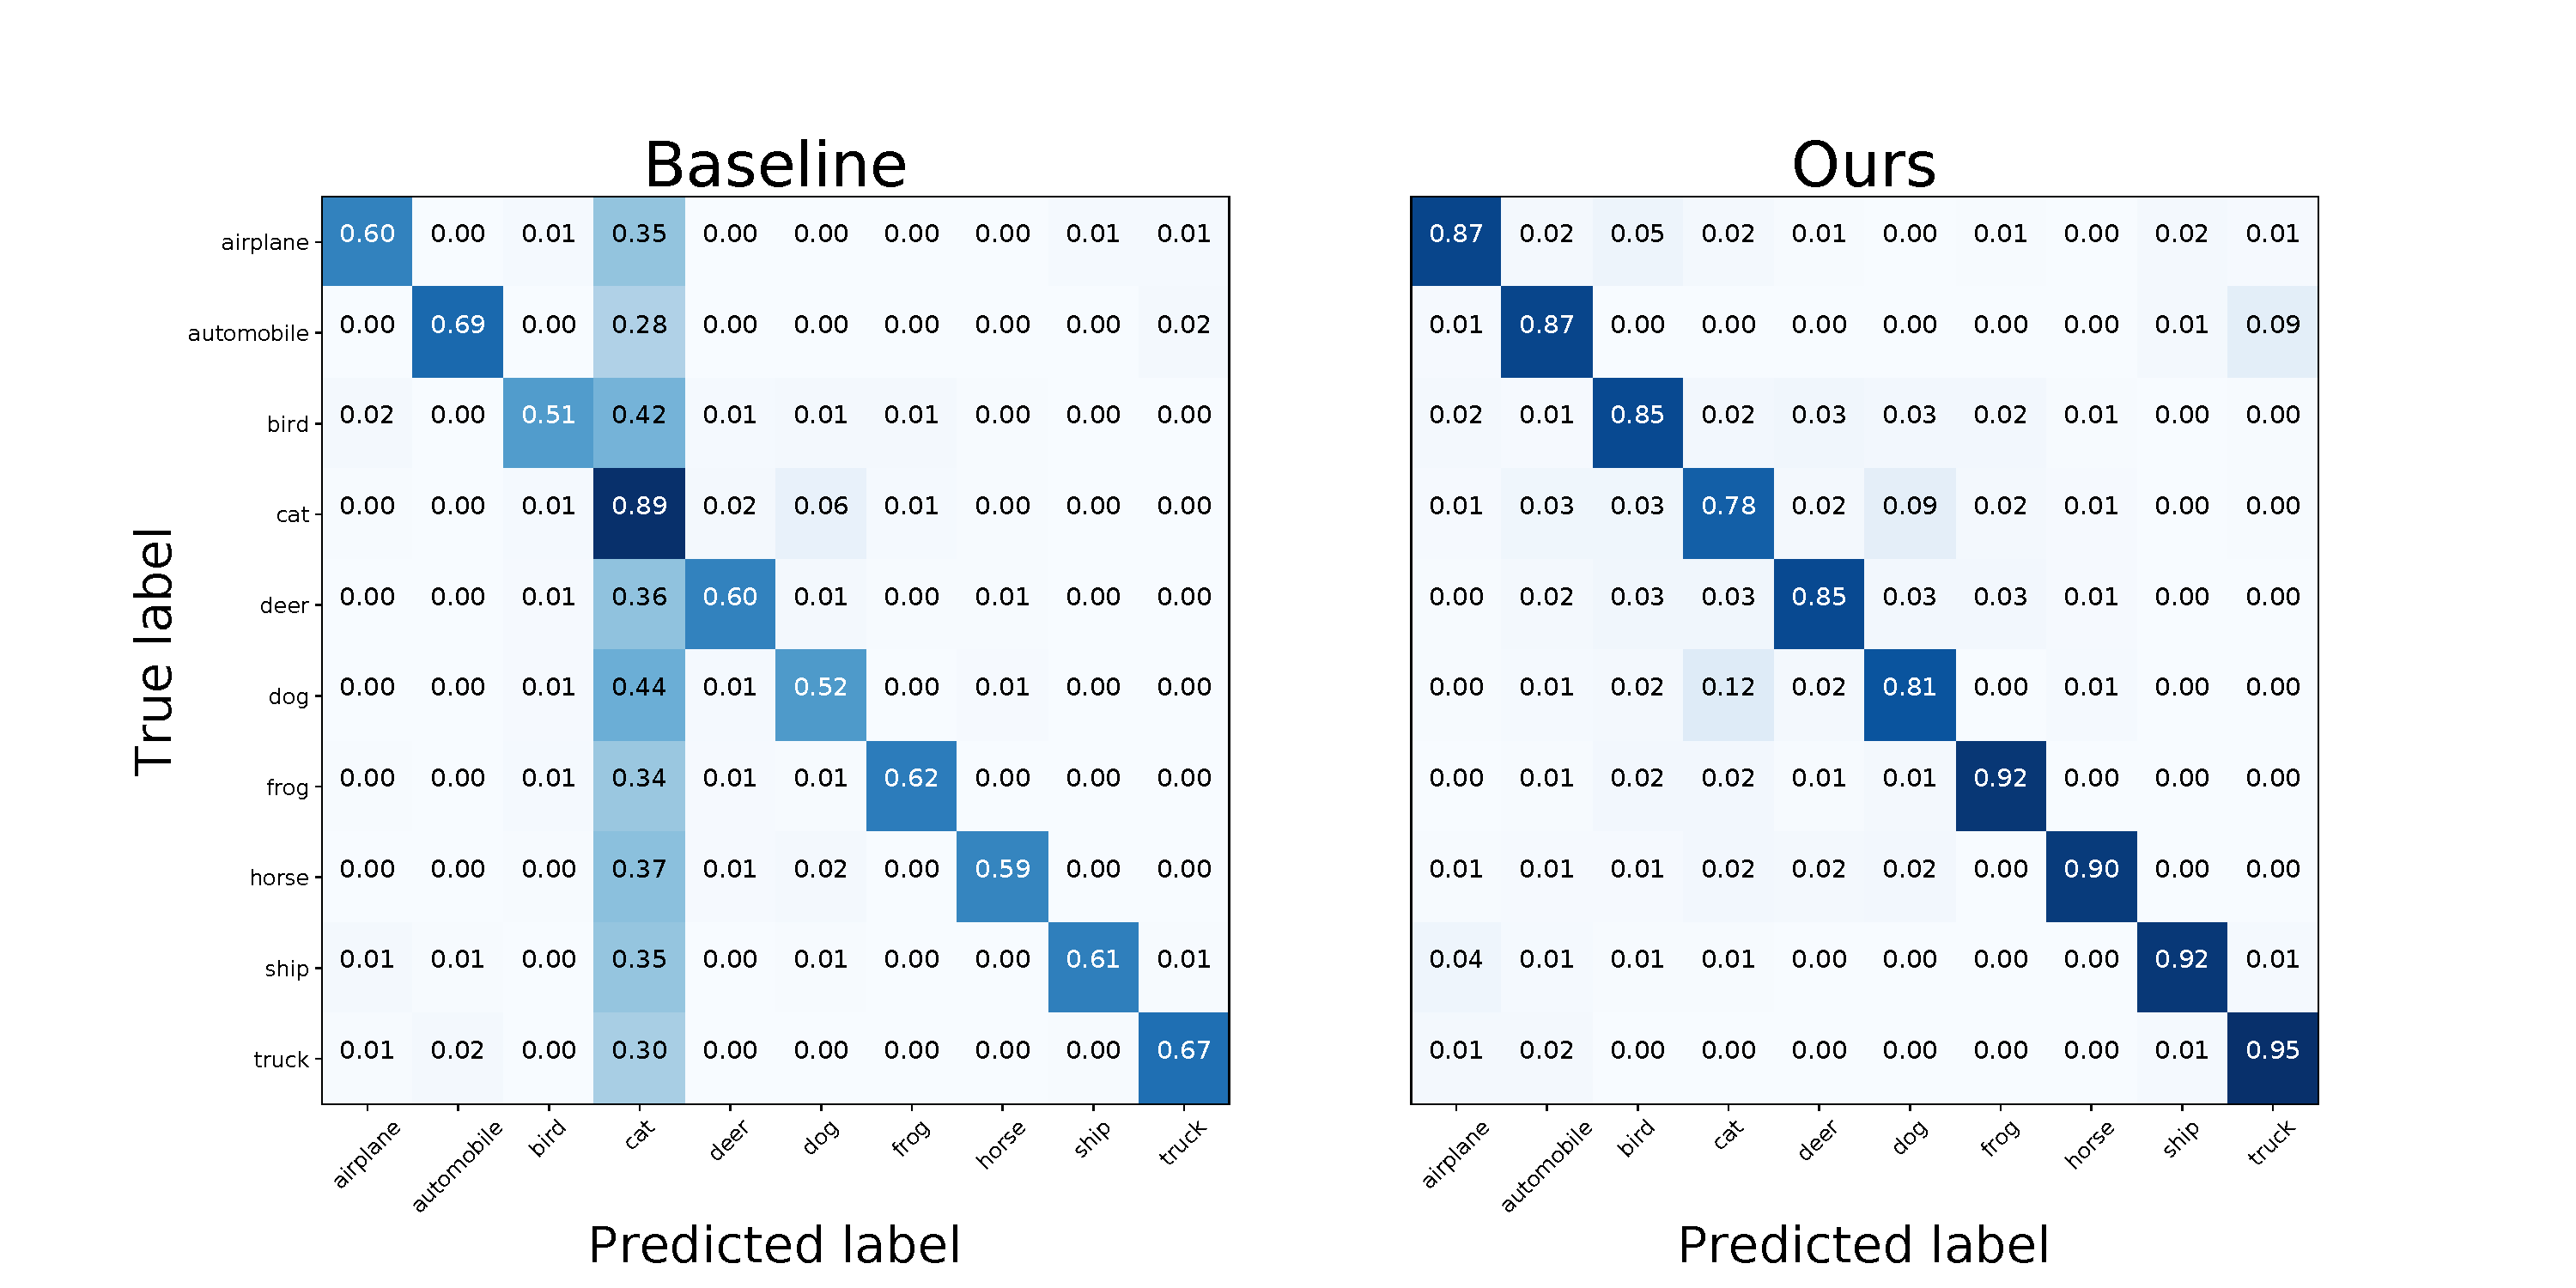
\includegraphics[width=\columnwidth,trim={2.5cm 0 4cm 0},clip]{figures/cifar-imbalance-cm.pdf}
\fi
\vspace{-0.2in}
\iflatexml
\caption{Confusion matrices on CIFAR-10 \textsc{UniformFlip} (left) and \textsc{BackgroundFlip} (right)}
\else
\caption{Confusion matrices on CIFAR-10 \textsc{UniformFlip} (top) and \textsc{BackgroundFlip} (bottom)}
\fi
\label{fig:confusion}
\vspace{-0.1in}
\end{figure}
